\documentclass{article}
\usepackage[a4paper, width=170mm, top=20mm, bottom=20mm]{geometry}
\usepackage{hyperref}
\usepackage{amsmath}
\usepackage{nopageno}
\usepackage{xcolor}
\usepackage{adjustbox}
\newcommand\tab[1][0.5cm]{\hspace*{#1}}
\usepackage{mdframed}
\newmdenv[linecolor=white,backgroundcolor=blue!10]{myframe}
\usepackage{graphicx}
\usepackage{subcaption}
\usepackage{amsmath}
\usepackage{bm}
\usepackage{lipsum}
\usepackage[shortlabels]{enumitem}
\usepackage{fancyhdr}
\pagestyle{fancy}
\renewcommand{\headrulewidth}{0pt}
\fancyhead{}
\fancyfoot{}
\fancyfoot[C]{\thepage}

% Set greek language
%\usepackage[english,greek]{babel}
\usepackage[utf8]{inputenc}
%\newcommand{\en}[1]{\foreignlanguage{english}{#1}}
%\usepackage{kerkis} 
%\usepackage{abc}

% Hyperref
\usepackage{hyperref}
\hypersetup{
	colorlinks=true,
	linkcolor=black,
	filecolor=black,      
	urlcolor=blue,
}

% Tables
\usepackage{tabu}
\usepackage{tabularx}
\newcolumntype{L}[1]{>{\raggedright\let\newline\\\arraybackslash\hspace{0pt}}m{#1}}
\newcolumntype{C}[1]{>{\centering\let\newline\\\arraybackslash\hspace{0pt}}m{#1}}
\newcolumntype{R}[1]{>{\raggedleft\let\newline\\\arraybackslash\hspace{0pt}}m{#1}}

\begin{document}
	

\noindent
\begin{huge}
\hspace{-3.0mm}\textbf{OpenFOAM Tutorials}
\end{huge}

\setcounter{section}{1}
\section{Add temperature to solvers}
	
\begin{enumerate}[2.1]
	\item Add  the heat transport equation to the {\tt icoFoam} solver, in order to calculate how the flow can affect the heat transfer between two heated walls. The heat transport equation is
	
	$$
	\dfrac{\partial T}{\partial t} + (\bm{V} \cdot \bm{\nabla}) T = \alpha \nabla^2 T
	$$

	where $\alpha$ is the themal diffusivity.
	
	Copy the {\tt icoFoam} solver to your OpenFOAM project directory, inside a folder named {\tt applications}, where you can store all your modified OpenFOAM solvers. If you haven't already created such directory, either do it manually, or follow the commands
	
	{\tt
		
	\tab	\$ mkdir -p \$WM\_PROJECT\_USER\_DIR/applications \\
	\tab 	\$ cp -r \$FOAM\_SOLVERS/incompressible/icoFoam \$WM\_PROJECT\_USER\_DIR/applications/myIcoFoam
	\tab 	\$ cd \$WM\_PROJECT\_USER\_DIR/applications/myIcoFoam
	}
	
	\vspace{0.2cm}
	
	Rename the {\tt icoFoam.C} file to {\tt myIcoFoam.C}. Now go into the Make subdirectory and open the 'files' file with a text editor. Change it to read: 


	\begin{myframe}
	{\tt %
	 myIcoFoam.C \\%
	 \\%	
	 EXE = \$(FOAM\_USER\_APPBIN)/myIcoFoam}
 	\end{myframe}


	You can delete old binaries, if they exist, using the command
	
	{\tt \tab \$ wclean}
	
	To compile the new solver, run the command
	
	{\tt \tab \$ wmake}
	
	If everything worked correctly, your new solver binary should be present in the {\tt FOAM\_USER\_APPBIN} directory. Check this with:
	
	{\tt \tab \$ ls \$FOAM\_USER\_APPBIN }
	
	\vspace{0.2cm}
	
	This will show the steps to add another field variable to a solver. Open the {\tt myIcoFoam.C} with a text editor. Following the flow of the {\tt myIcoFoam} program, one notices that the header file {\tt createFields.H} is called prior to the solution loop. This file was copied with the solver and has the specific information pertaining to what variables will be solved. Inside the {\tt createFields.H} file, the first items loaded is the kinematic viscosity from the {\tt transportProperties} dictionary file. We will add a new transport property related to the thermal diffusivity which will be denoted as {\tt alpha}. Make the following edits: 
	

	\begin{myframe}
	{\tt %
 
		Info<< "Reading transportProperties\textbackslash n" << endl;
		\\
		
		IOdictionary transportProperties \\
		(\\
		\tab IOobject \\
		\tab ( \\
		\tab \tab "transportProperties",\\
		\tab \tab runTime.constant(), \\
		\tab \tab mesh,\\
		\tab \tab IOobject::MUST\_READ,\\
		\tab \tab IOobject::NO\_WRITE\\
		\tab )\\
		 );
		\\
		
		dimensionedScalar nu \\
		( \\
		\tab transportProperties.lookup("nu") \\
		);\\
		//Add here... \\
		dimensionedScalar alpha \\
		(\\
		\tab transportProperties.lookup("alpha")\\
		);\\
		//Done for now... \\

	}
	\end{myframe}

	Later on, we will need to edit the {\tt transportProperties} dictionary file to reflect this change. Moreover, in the same file, add a {\tt volScalarField}, similar to the pressure field, that represents the temperature.
	
	\begin{myframe}
	{\tt %
		
		Info<< "Reading field T\textbackslash n" <<endl; \\
		\\
		volScalarField T\\
		(\\
		\tab IOobject \\
		\tab ( \\
		\tab \tab "T",\\
		\tab \tab runTime.timeName(),\\
		\tab \tab mesh,\\
		\tab \tab IOobject::MUST\_READ,\\
		\tab \tab IOobject::AUTO\_WRITE\\
		\tab ),\\
		\tab mesh \\
		);\\
			
	}
	\end{myframe}
	
	Save these changes. You've completed adding a new scalar field variable 'T' and a new constant 'alpha'.
	
	The next step is to add a new equation describing the transport of the temperature. Return to editing the {\tt myIcoFoam.C} file. Because the temperature transport depends on the velocity field, we will add the equation after the momentum equation is solved (after the PISO loop), but before the time step is written. Edit your file so it looks like this: 
	

	\begin{myframe}
	{\tt %
		
		\tab\tab\tab \#include "continuityErrs.H" \\
		\\
		\tab\tab\tab U -= rUA*fvc::grad(p);\\
		\tab\tab\tab U.correctBoundaryConditions();\\
		\tab\tab \}\\
		\\
		\tab\tab //add these lines...\\
		\tab\tab fvScalarMatrix TEqn\\
		\tab\tab (\\
		\tab\tab\tab fvm::ddt(T)\\
		\tab\tab\tab + fvm::div(phi, T)\\
		\tab\tab\tab - fvm::laplacian(alpha, T)\\
		\tab\tab);\\
		\\
		\tab\tab TEqn.solve();\\
		\tab\tab //done adding lines...\\
		\\
		\tab\tab runTime.write();\\
	}
	\end{myframe}
	
	These lines add a new equation for the temperature and make use of the face flux variable, phi, which is already used in the momentum equation solution.
	
	Save your changes and run wmake to compile the solver: 
		
	{\tt \tab \$ wmake}
	
	
	
	\item The next step in this process is to test the new solver. This will first be accomplished by modifying the existing cavity tutorial. Copy a cavity case from the tutorials folder into your OpenFOAM directory. Open the {\tt transportProperties} dictionary in your favorite editor and add the following line under the definition of nu: 
	
	\begin{myframe}
	{\tt %
	alpha \tab \tab \tab alpha [0 2 -1 0 0 0 0] 0.002;
	}
	\end{myframe}
	
	
	In the {\tt ./0/} folder, create a file for the initial and boundary conditions of temperature:
	
	\begin{myframe}
	{\tt %

	FoamFile\\
	\{\\
		\tab version\tab ~~~ 2.0;\\
		\tab format\tab ~~~~ ascii;\\
		\tab class\tab ~~~~~ volScalarField; \\
		\tab object\tab ~~~~ T; \\
	\} \\
	//**********************************// \\
	\\
	dimensions\tab\tab ~~~~~ [0 0 0 1 0 0 0];\\
	\\
	internalField\tab\tab ~~  uniform 300;\\
	\\
	boundaryField\\
	\{\\
	\tab movingWall\\
	\tab \{\\
		\tab \tab type \tab \tab   \tab ~~  fixedValue;\\
		\tab \tab value \tab \tab   \tab ~  uniform 350;\\
	\tab \}\\
	\\
	\tab fixedWalls\\
	\tab \{\\
		\tab \tab type    \tab \tab \tab  ~~ fixedValue;\\
		\tab \tab value  \tab \tab \tab  ~  uniform 300;\\
	\tab\}\\
	\\
	\tab frontAndBack\\
	\tab \{\\
		\tab \tab type   \tab \tab \tab   ~~  empty;\\
	\tab \}\\
	\}\\
	
	}
\end{myframe}
	
	
	The next thing tha must be done is to choose discretization scemes and solution algorithms for the extra energy equation. By adding a new equation to solve, we need to tell OpenFOAM what discretization schemes to apply to the equations. This is done in the {\tt fvSchemes} dictionary. Open the 'fvSchemes' dictionary. Now, there are two main items added in the thermal transport equation above: a divergence term and a laplacian. Under each of these sections in the dictionary, we need to add terms which match what was added in the solver source code. Edit your file so it includes the following: 
	
	\begin{myframe}
	{\tt %
	divSchemes\\
	\{\\
	\tab default~~~~~~~~~~~~~~~~none;\\
	\tab div(phi,U)~~~~~~~~~~~~~Gauss linear; \\
	\tab div(phi,T)~~~~~~~~~~~~~Gauss upwind; \\
	\}\\
	\\
	laplacianSchemes\\
	\{\\
	\tab default~~~~~~~~~~~~~~~~none;\\
	\tab laplacian(nu,U)~~~~~~~~Gauss linear corrected;\\
	\tab laplacian((1|A(U)),p)~~Gauss linear corrected;\\
	\tab laplacian(alpha,T)~~~~~Gauss linear corrected;\\
	\}\\
		
	}
	\end{myframe}

	Alternatively, a scheme can be added to the 'default' field instead of adding specific ones below. Next, open the {\tt fvSolution} dictionary. It should look like this: 
	
	\begin{myframe}
	{\tt %
	solvers\\
	\{\\
    \tab  p\\
	\tab \{\\
	\tab \tab solver~~~~~~~~~~~~PCG;\\
	\tab \tab preconditioner~~~~DIC;\\
	\tab \tab tolerance~~~~~~~~~1e-06;\\
	\tab \tab relTol~~~~~~~~~~~~0.05;\\
	\tab \}\\
	\\
	\tab pFinal\\
	\tab \{\\
	\tab \tab\$p;\\
	\tab \tab relTol~~~~~~~~~~~~0;\\
	\tab \}\\
	\\
	\tab U\\
	\tab \{\\
	\tab \tab solver~~~~~~~~~~~~smoothSolver;\\
	\tab \tab smoother~~~~~~~~~~symGaussSeidel;\\
	\tab \tab tolerance~~~~~~~~~1e-05;\\
	\tab \tab relTol~~~~~~~~~~~~0;\\
	\tab \}\\
	\tab //add this...\\
	\tab T \\
	\tab \{\\
	\tab \tab solver~~~~~~~~~~~~BICCG;\\
	\tab \tab preconditioner~~~~DILU;\\
	\tab \tab tolerance~~~~~~~~~1e-7;\\
	\tab \tab relTol~~~~~~~~~~~~0;\\
	\tab \};\\
	\tab //done editing...\\
	\}
	}
	\end{myframe}


	After successfully running the case, the temperature field should look similar to the following picture
	
	\begin{center}
		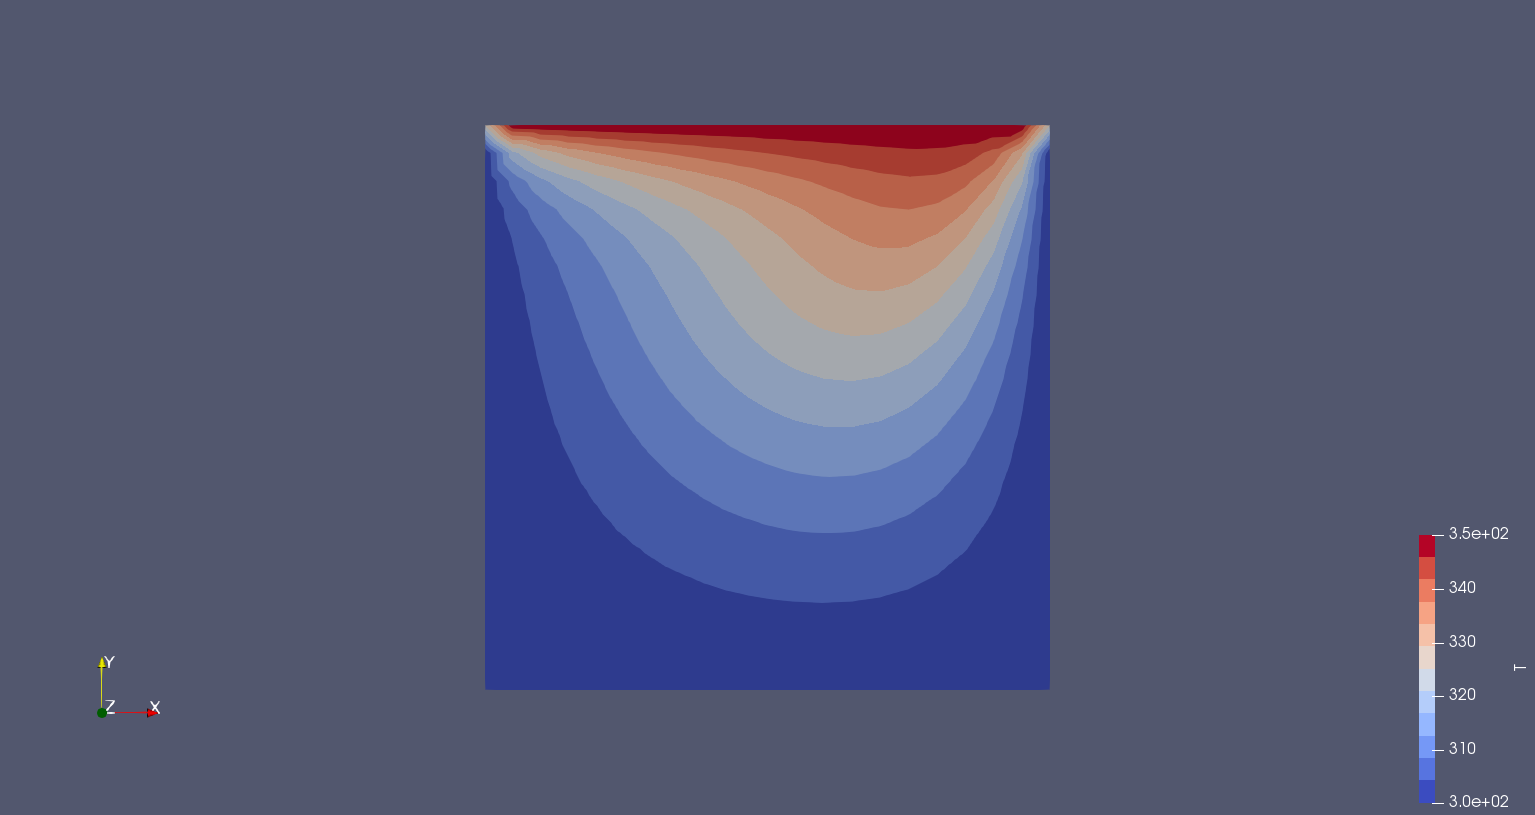
\includegraphics[width = 0.8\textwidth]{temp.png}
	\end{center}
	
	
	\item Simulate the thermal laminar 3D pipe flow of the previous tutorial, by adding a temperature field, similarly with the previous step. Define two opposite walls with temperatures 300 K and 350 K respectively, while the other two will be fully insulated.
	
	\item Create a new solver, called {\tt laplaceFoam} that solves the Laplace equation in a rectangular flat plate, with boundary and initial conditions as shown in the next figure. Use the quantities $T_w=100~K,~L=2~m$ and $H=1~m$.
	
	
	\begin{center}
		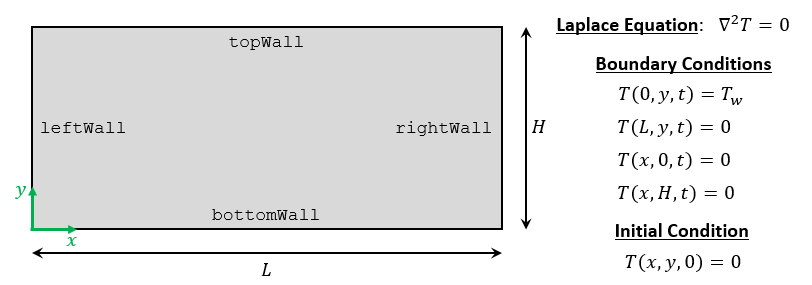
\includegraphics[width=0.8\textwidth]{laplace.png}
	\end{center}

	For the creation of the new solver, copy the existing solver {\tt electrostaticFoam} into the {\tt applications} directory, in your {\tt Home} folder, and change the name in all the appropriate files, as described in Step 2.

	Modify the {\tt laplaceFoam.C} and the  {\tt createFields.H} files, in order to only solve the Laplace equation for the {\tt volScalarField} T. Delete any unnecessary commands, equations and variables inside the solver and compile the solver.

	Create the case and test the validity of your results.

	
\end{enumerate}

%	
%	\item Σε αυτό το βήμα θα μοντελοποιηθεί η μετάδοση θερμότητας σε δυο εφαπτομενικά  χωρία, το ένα θα είναι μία στερεή πλάκα, όπου θα λυθεί η εξίσωση \en{Laplace} και το άλλο ο αέρας, όπου θα λυθεί η εξίσωση \en{Poisson}. Στο παρακάτω σχήμα φαίνονται ακριβώς τα χαρακτηριστικά, οι εξισώσεις και οι συνοριακές συνθήκες που θα χρησιμοποιηθούν. Μπορεί να χρησιμοποιηθεί ο λύτης \en{\tt laplaceFoam} που ήδη έχετε κατασκευάσει στο προηγούμενο βήμα, και να τροποποιηθεί για το συγκεκριμένο πρόβλημα.
%	
%	\begin{center}
%		\includegraphics[scale = 0.5]{regions.jpg}
%	\end{center}
%	
%	Για να επιτευχθεί αυτό, θα πρέπει να δημιουργηθεί ένα \en{block} στο μέγεθος και των δύο χωρίων από το \en{\tt blockMeshDict}, και μετά χρησιμοποιώντας το εργαλείο \en{\tt topoSet} του \en{OpenFOAM} να χωριστούν σε δύο \en{regions}. Το ένα \en{region} να ονομαστεί \en{solid} και το άλλο \en{air}. Στην διεπιφάνεια των δύο \en{regions} θα πρέπει να οριστούν κατάλληλες οριακές συνθήκες για την σωστή λύση των εξισώσεων. Πιο συγκεκριμένα, θα πρέπει η τιμή της θερμοκρασίας και η παράγωγός της στο \en{interface} των δύο περιοχών να είναι ίσες
%	
%	$$ T_{air} = T_{solid} $$
%	
%	$$ k_{air} \dfrac{\partial T}{\partial n} \Bigg|_{air} = k_{solid} \dfrac{\partial T}{\partial n} \Bigg|_{solid} $$
%	
%	όπου $k$ είναι ο συντελεστής θερμικής αγωγιμότητας του κάθε χωρίου.
%	
%	Η οριακή συνθήκη που χρησιμοποιείται είναι η:
%	
%	\tab \en{\tt compressible::turbulentTemperatureCoupledBaffleMixed}
%
%	και μπορεί να βρεθεί ο τρόπος χρήσης της, όπως και ο τρόπος δημιουργίας \en{regions} με το \en{\tt topoSet} (αρχείο \en{\tt topoSetDict}), από τα \en{tutorial cases} του λύτη \en{\tt chtMultiRegionFoam}, που βρίσκεται στην κατηγορία \en{heat transfer}. 
%	
%	Επιπλέον, θα πρέπει να δημιουργηθούν στον \en{solver} δύο διαφορετικά πλέγματα, όπου στο ένα (\en{meshA}) θα λυθεί η εξίσωση \en{Poisson} για τον αέρα και στο άλλο (\en{meshS}) θα λυθεί η εξίσωση \en{Laplace} στο στερεό. Αυτό συνεπάγεται, πως θα υπάρχουν δύο διαφορετικές μεταβλητές (\en{\tt scalarFields}) στο αρχείο \en{\tt createFields.h}, μία για την θερμοκρασία στον αέρα \en{\tt Tair} και μία για την θερμοκρασία στο στερεό \en{\tt Tsolid}. Αντίστοιχα, όπως αναφέρθηκε προηγουμένως, θα πρέπει να υπάρχουν δύο διαφορετικές εξισώσεις στο αρχείο \en{\tt laplaceFoam.c}, η \en{Poisson} για την \en{\tt Tair} στο \en{meshA}, και η \en{Laplace} για την \en{\tt Tsolid} στο \en{meshS}.
%	
%	Θα πρέπει να υπάρχουν, αντίστοιχα και στο \en{case} δύο διαφορετικά αρχεία για τις συνοριακές συνθήκες και να τοποθετηθούν στους φακέλους που θα δημιουργηθούν μετά την χρήση του \en{\tt topoSet}, στις διαδρομές \en{\tt ./0/air} και \en{\tt ./0/solid} . Σε κάθε αρχείο συνοριακής συνθήκης θα πρέπει να προστεθεί και η συνθήκη για την διεπιφάνεια. Ο ακριβής τίτλος του συνόρου των διεπιφανειών (μία για κάθε \en{region}) δημιουργείται αυτόματα από την εντολή \en{\tt topoSet} και μπορεί να βρεθεί στις διαδρομές \en{\tt ./constant/air} και \en{\tt ./constant/solid}. Τέλος, πρέπει να σημειωθεί, πως για την σωστή λειτουργία της συνοριακής συνθήκης \en{\tt BaffleMixed} θα πρέπει να δημιουργηθούν δυο \en{scalar} μεταβλητές π.χ. \en{kappaA} και \en{kappaS} οι οποίες θα έχουν την τιμή των σταθερών $k_{air}$ και $k_{solid}$ σε ολόκληρο το \en{region} που αντιστοιχεί σε κάθε μεταβλητή.
%	
%	Παράδειγμα της συνοριακής συνθήκης για την μεταβλητή \en{\tt Tair} φαίνεται παρακάτω.
%	
%	\hspace{0.4cm}
%	\begin{minipage}{0.92\textwidth}
%	\begin{myframe}
%	\en{\tt %
%    air\_to\_solid\\%
%		\{\\%
%		\tab	type  ~~~~~~~~~~          compressible::turbulentTemperatureCoupledBaffleMixed;\\%
%		\tab	value  ~~~~~~~~~         \$internalField;\\%
%		\tab	Tnbr   ~~~~~~~~~~         Tsolid;\\%
%		\tab	kappaMethod ~~~    lookup;\\%
%		\tab	kappa    ~~~~~~~~~       kappaA;\\%
%		\}\\%
%	}
%	\end{myframe}
%	\end{minipage}
%	
%	
%	
%	
%	
%	
%	
%
%	
%	
%\end{enumerate}










\end{document}